\qs{}{
    How many courses are held in all the buildings?
}

This creates a view that selects the unique course code and building values from the course table using the DISTINCT keyword and then counts the number of courses grouped by the name of the building. 
\vspace{\baselineskip}

\sol{}
\noindent\line(1, 0){0.89\linewidth}
\begin{verbatim}
CREATE VIEW crs_bldg_base AS
SELECT DISTINCT crs_code, crs_bldg_name
FROM course;

SELECT crs_bldg_name AS "Building Name", COUNT(*) AS "Number of Courses Held"
FROM crs_bldg_base
GROUP BY crs_bldg_name;
\end{verbatim}
\noindent\line(1, 0){\linewidth}

\begin{figure}[H]
    \centering
    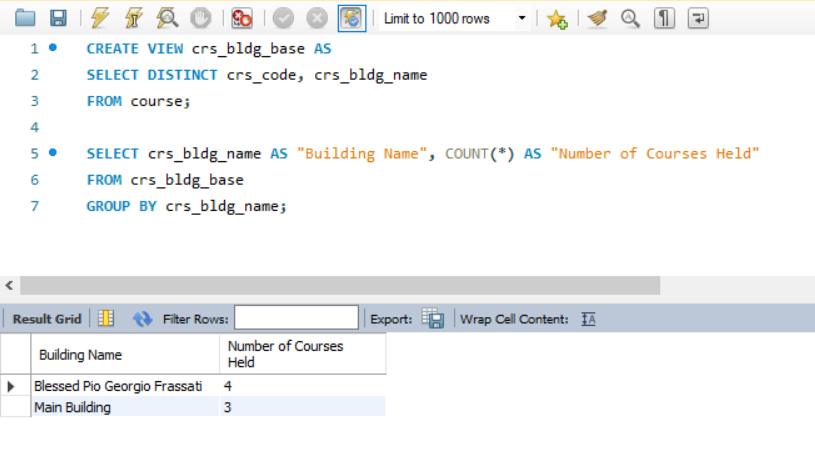
\includegraphics[width=0.7\linewidth]{images/q8.png}
    \caption{Question 8 Query and Output}
\end{figure}
